% -------------------------------------------------------------------------
\section{Applications}\label{sec:applications}
% -------------------------------------------------------------------------

We apply the new and original versions of lookout to two real datasets. Neither has labelled anomalies, so accuracy cannot be measured, but both have two variables, so the output can be inspected.
\begin{enumerate}
  \item Old Faithful dataset\footnote{Data downloaded from \url{https://geysertimes.org}.}: 2,097 eruptions of the Old Faithful Geyser in Yellowstone National Park, Wyoming, USA, from 14 January 2017 to 29 December 2023. For each recorded eruption the duration is given in seconds along with the waiting time to the following eruption. The records are incomplete, especially during winter.
  \item Wine reviews dataset\footnote{Data downloaded from \url{https://www.kaggle.com/datasets/zynicide/wine-reviews/data}.}: 110,203 reviews of wines from 42 countries, obtained from the \emph{Wine Enthusiast Magazine} during the week of 15 June 2017. We use the 4,496 wines labelled Shiraz or Syrah, and two variables: the points score given by the \emph{Wine Enthusiast} reviewer on a scale of 0--100, and the price of a bottle. The kernel density estimates use the truncated sum described in \cref{sec:modified}, with 100 neighbours.
\end{enumerate}

\begin{figure}[!htb]
  \centering
  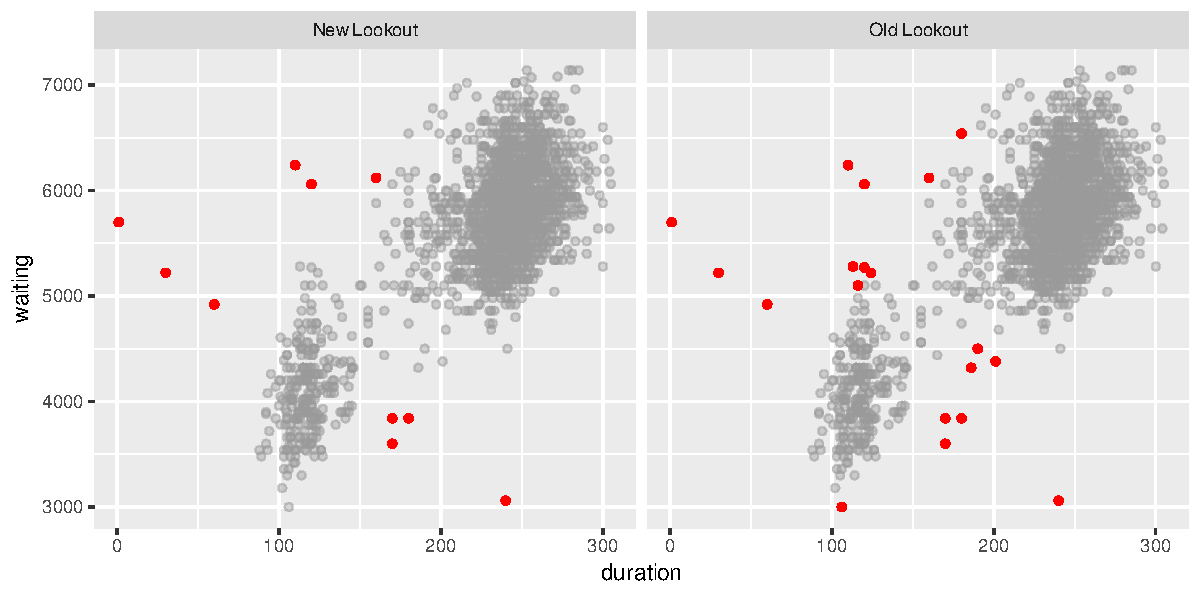
\includegraphics[width=0.8\linewidth]{Figures/old_faithful.pdf}
  \caption{Anomalies (red) identified in the Old Faithful data by the new version of lookout (left) and the original version (right).}
  \label{fig:oldfaithful}
\end{figure}

\begin{figure}[!htb]
  \centering
  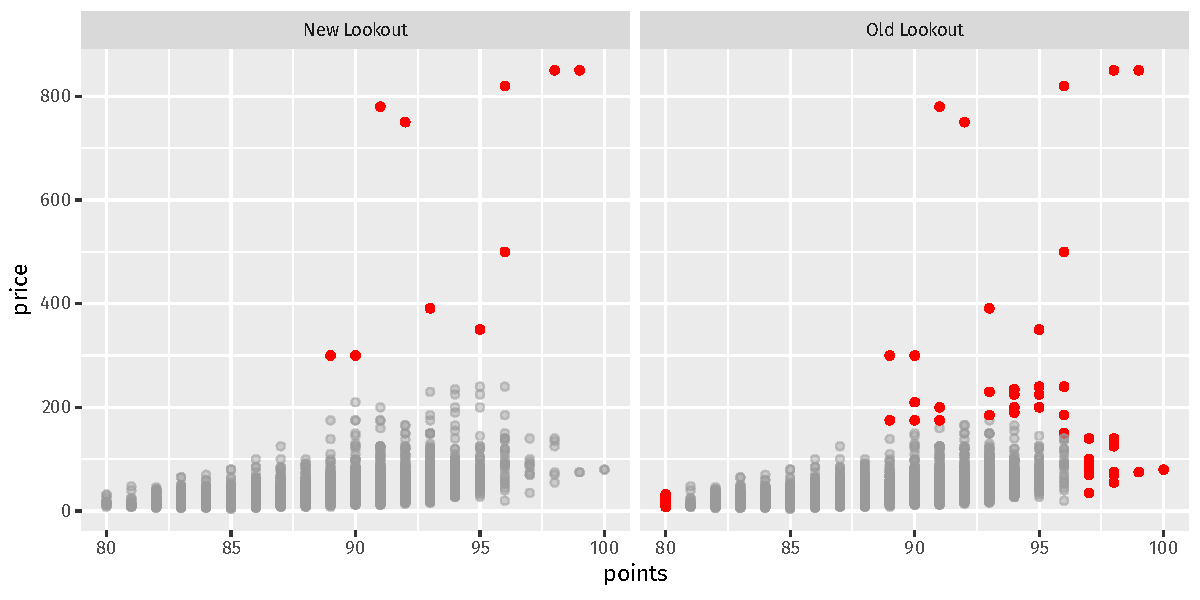
\includegraphics[width=0.8\linewidth]{Figures/wine_reviews.pdf}
  \caption{Anomalies (red) identified in the wine reviews data by the new version of lookout (left) and the original version (right).}
  \label{fig:winereviews}
\end{figure}

\cref{fig:oldfaithful} shows the Old Faithful data. The new version identifies the observations in the sparse regions between and around the two clusters. The original identifies fewer of those, and instead flags a group of observations at the lower edge of the smaller cluster, close to the bulk of the data.

\cref{fig:winereviews} shows the wine reviews. The new version identifies the expensive wines and little else. The original also flags many wines with the highest and lowest scores at ordinary prices, and several at the edge of the main cloud. In both datasets the new version flags the observations that are isolated in the two-dimensional space, and the original flags observations at the margins of the dense regions as well; we regard the former as the more useful behaviour.
